\section{Movimiento en dos dimensiones}
  \subsection{Vectores de posición, velocidad y aceleración}
    \PN En dos dimensiones, la posición de una partícula se indica mediante su vector de posición $\BV{r}$, que se
    dibuja desde el origen de algún sistema coordenado a la posición de la partícula en el plano xy.

    \begin{figure}[H]
      \centering
      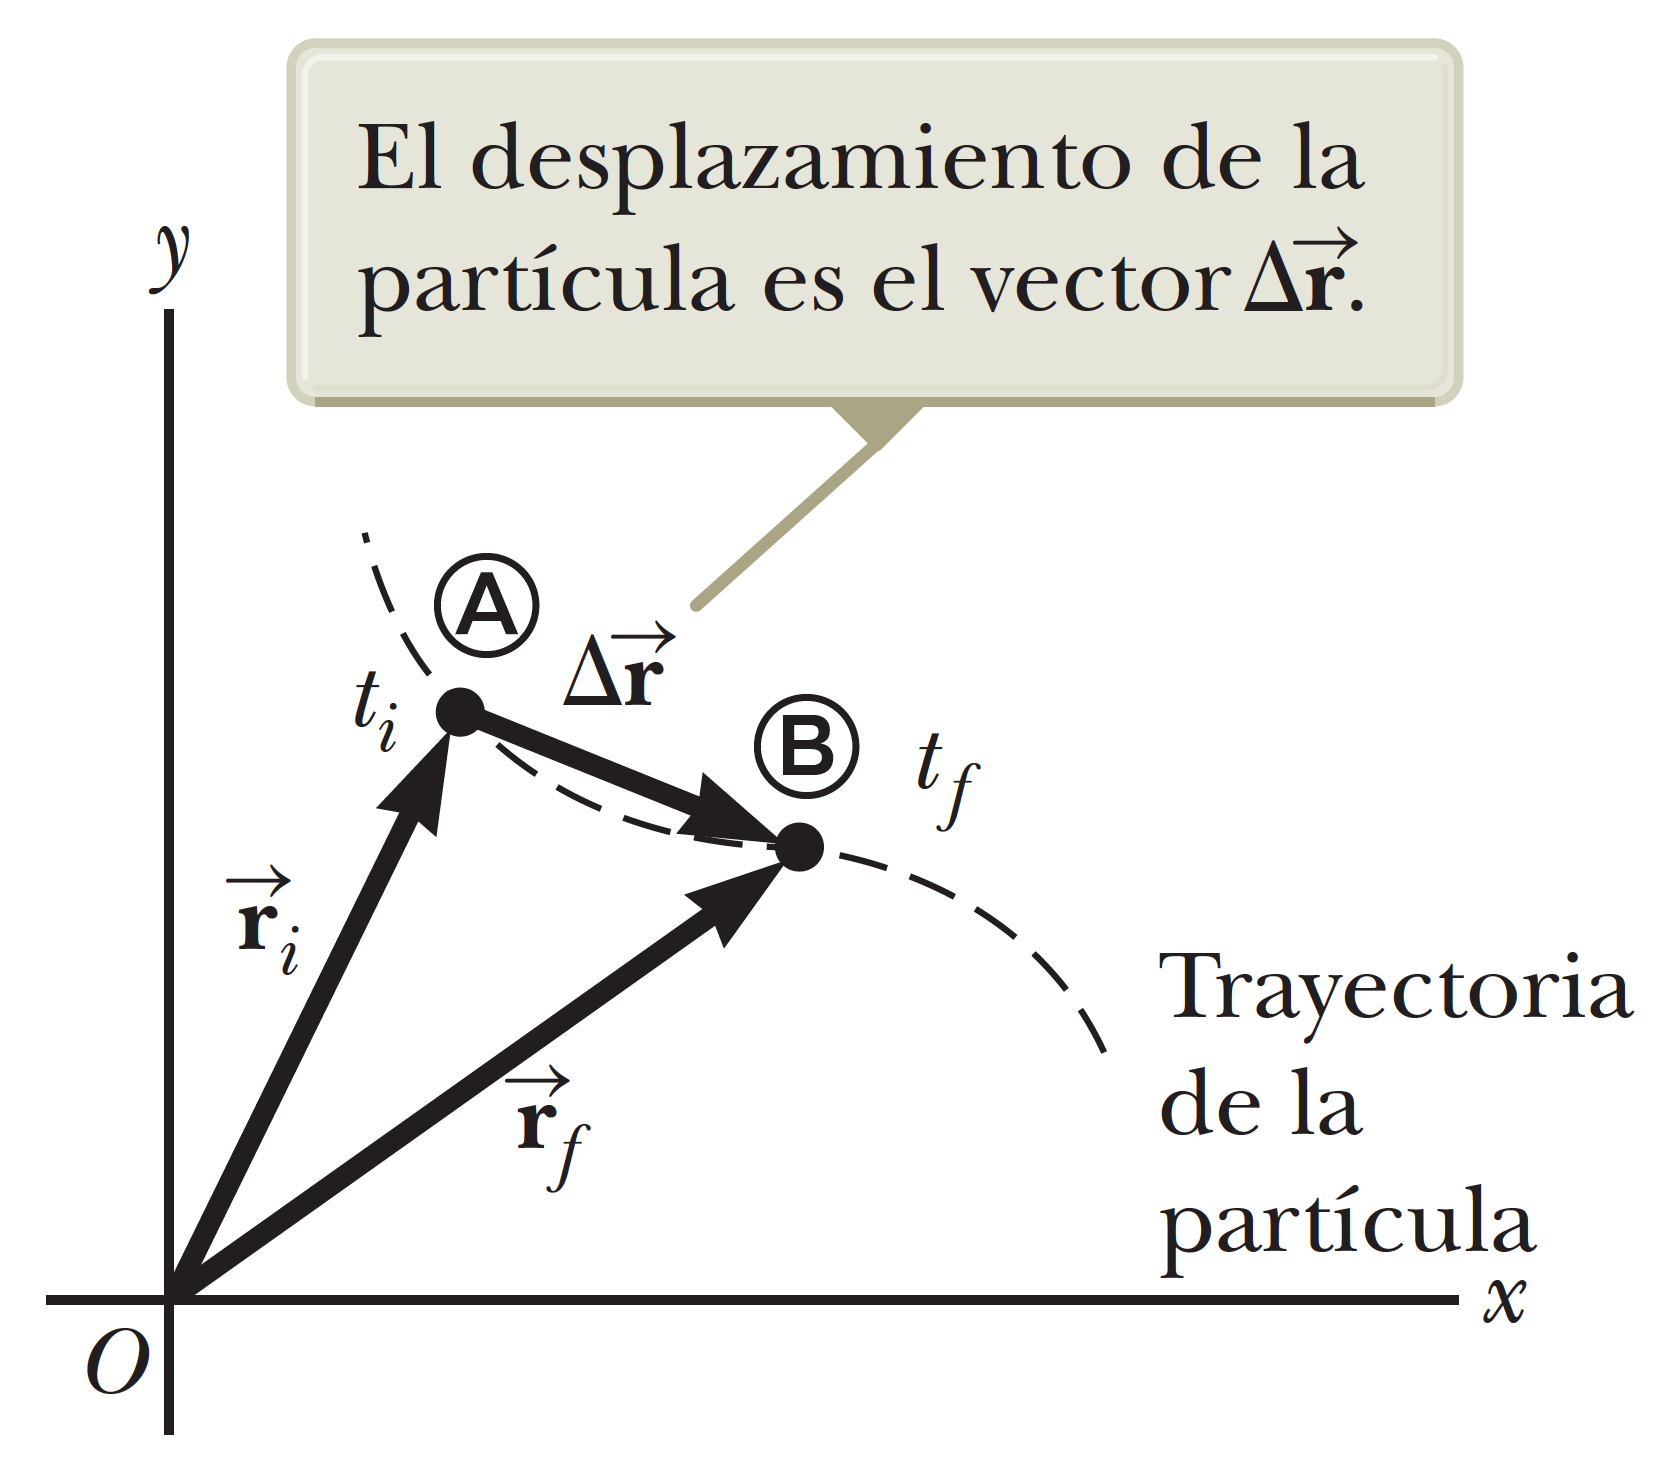
\includegraphics[scale=0.2]{1/graphics_4/figure_0}
      \caption{Una partícula que se mueve en el plano xy se ubica con el vector de posición $\BV{r}$, que se dibuja
      desde el origen hasta la partícula.}
    \end{figure}

    \begin{itemize}
      \item El \textbf{vector desplazamiento} $\BV{r}$ para una partícula se define como la diferencia entre su vector
      de posición final y su vector de posición inicial:
        \begin{equation*}
          \Delta \BV{r} = \BV{r}_{f} - \BV{r}_{i}
        \end{equation*}

      \item La \textbf{velocidad promedio} $\BV{v}_{prom}$ de una partícula durante el intervalo de tiempo $\Delta t$ se
      define como el desplazamiento de la partícula dividido entre el intervalo de tiempo:
        \begin{equation*}
          \BV{v}_{prom} \equiv \frac{\Delta \BV{r}}{\Delta t}
        \end{equation*}

        \PN Al multiplicar o dividir una cantidad vectorial por una cantidad escalar positiva como $\Delta t$ sólo
        cambia la magnitud del vector, no su dirección.

      \item La \textbf{velocidad instantánea} $\BV{v}$ se define como el límite de la velocidad promedio $\Delta \BV{r}$
      / $\Delta t$ conforme $\Delta t$ tiende a cero:
        \begin{equation*}
          \BV{v} \equiv \lim_{\Delta t \rightarrow 0} \ \frac{\Delta \BV{r}}{\Delta t} = \frac{d \BV{r}}{dt}
        \end{equation*}

        \PN Esto es, la velocidad instantánea es igual a la derivada del vector de posición respecto del tiempo.

        \PN La magnitud del vector velocidad instantánea $ v = \abs{\BV{v}}$ de una partícula se llama \textit{rapidez}
        de la partícula, que es una cantidad escalar.

      \item La \textbf{aceleración promedio} $\BV{a}_{prom}$ de una partícula se define como el cambio en su vector
      velocidad instantánea $\Delta \BV{v}$ dividido entre el intervalo de tiempo $\Delta t$ durante el que ocurre dicho
      cambio:
        \begin{equation*}
          \BV{a}_{prom} \equiv \frac{\Delta \BV{v}}{\Delta t} = \frac{\BV{v}_{f} - \BV{v}_{i}}{t_{f} - t_{i}}
        \end{equation*}

      \item La \textbf{aceleración instantánea} $\BV{a}$ se define como el valor límite de la razón $\Delta \BV{v}$ /
      $\Delta t$ conforme $\Delta t$ tiende a cero:
        \begin{equation*}
          \BV{a} \equiv \lim_{\Delta t \rightarrow 0} \ \frac{\Delta \BV{v}}{\Delta t} = \frac{d \BV{v}}{dt}
        \end{equation*}
    \end{itemize}

  \subsection{Movimiento en dos dimensiones con aceleración constante}
    \PN El movimiento en dos dimensiones se puede representar como dos movimientos independientes en cada una de las
    dos direcciones perpendiculares asociadas con los ejes x e y. Esto es: cualquier influencia en la dirección y no
    afecta el movimiento en la dirección x y viceversa.

    \PN El vector de posición para una partícula que se mueve en el plano xy se puede escribir
    \begin{equation*}
      \BV{r} = x \mathbf{\hat{i}} + y \mathbf{\hat{j}}
    \end{equation*}

    \PN donde x, y y $\BV{r}$ cambian con el tiempo a medida que la partícula se mueve mientras los vectores unitarios
    $\mathbf{\hat{i}}$ y $\mathbf{\hat{j}}$ permanecen constantes.

    \begin{figure}[H]
      \centering
      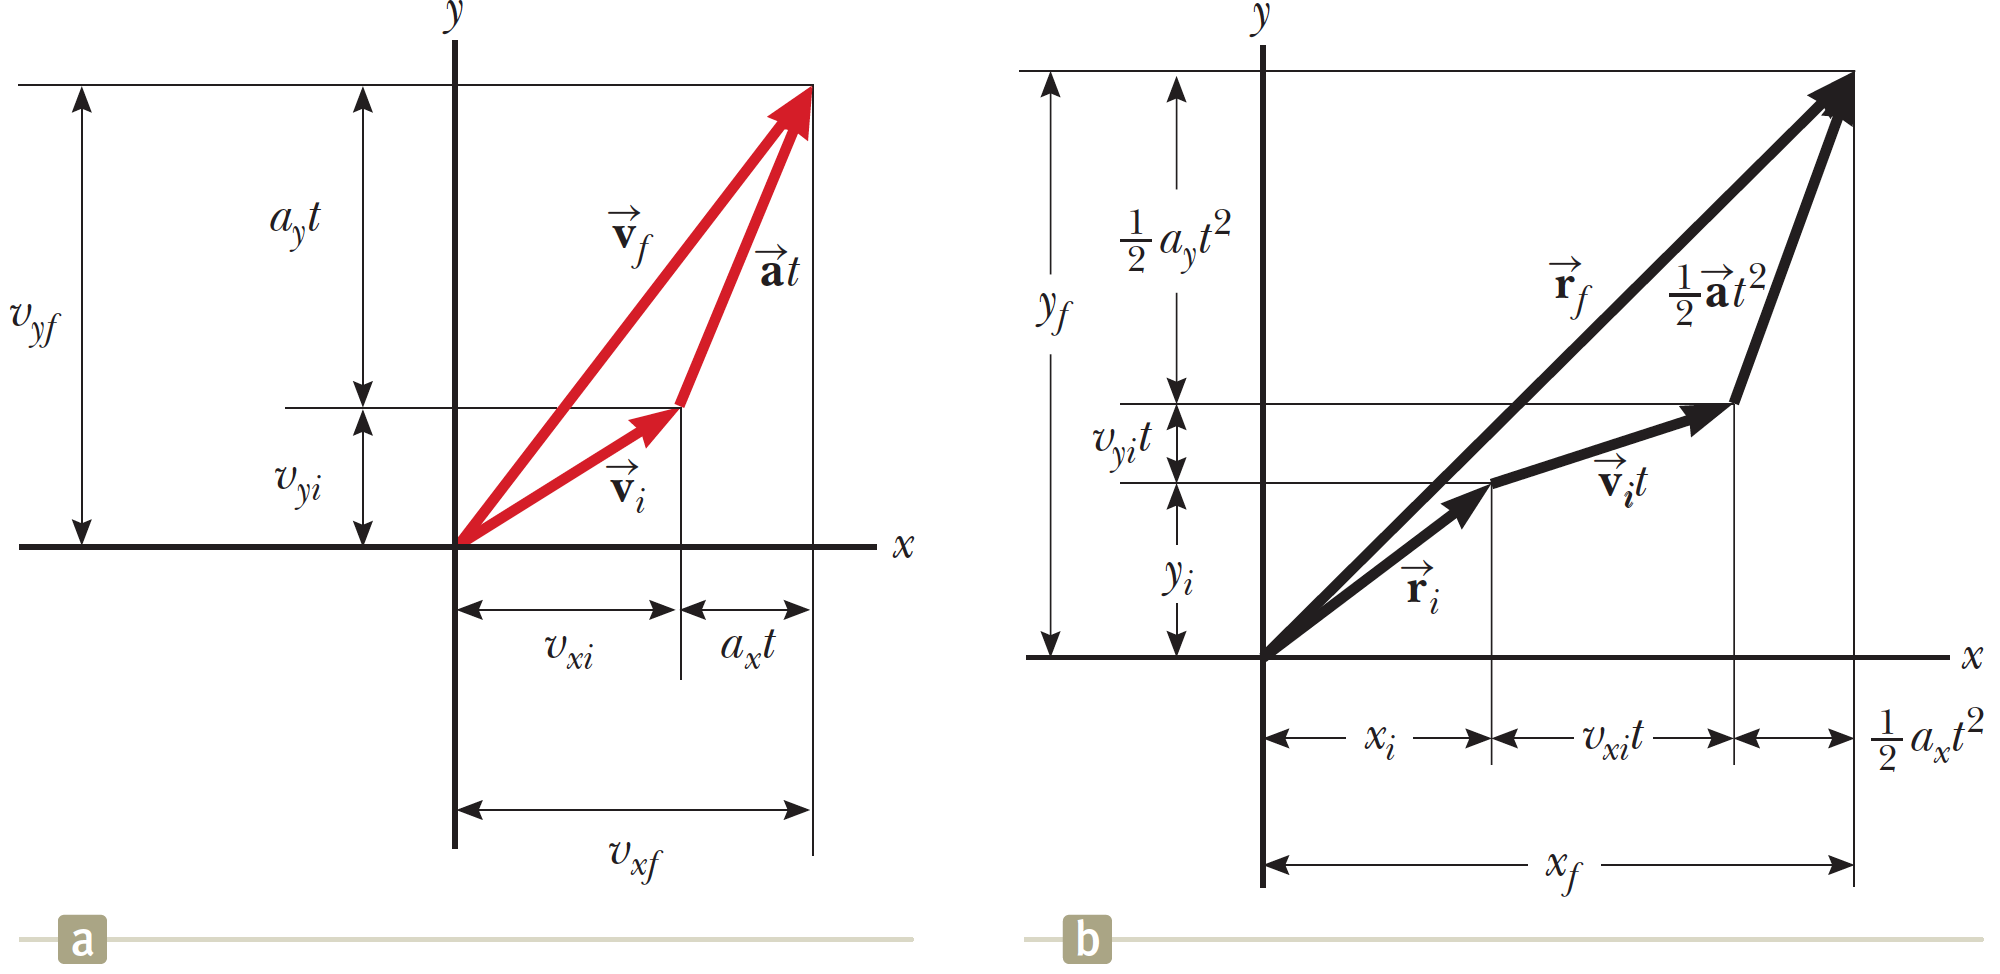
\includegraphics[scale=0.4]{1/graphics_4/figure_1}
      \caption{(a) Gráfico de vector velocidad: $\BV{v}_{f} = \BV{v}_{i} + \BV{a} t$. (b) Gráfico del vector posición:
      $\BV{r}_{f} = \BV{r}_{i} + \BV{v}_{i} t + \frac{1}{2} \BV{a} t^{2}$.}
    \end{figure}

  \subsection{Movimiento de un proyectil}
    \PN El \textbf{movimiento de proyectil} de un objeto es simple de analizar a partir de dos suposiciones:
    \begin{enumerate}
      \item La aceleración de caída libre es constante en el intervalo de movimiento y se dirige hacia abajo
      \item El efecto de la resistencia del aire es despreciable
    \end{enumerate}

    \PN La expresión para el vector de posición del proyectil como función del tiempo, siendo su aceleración la de la
    gravedad, $\BV{a} = \BV{g}$ es:
    \begin{equation*}
      \BV{r}_{f} = \BV{r}_{i} + \BV{v}_{i} t + \frac{1}{2} \BV{g} t^{2}
    \end{equation*}

    \PN donde las componentes x e y de la velocidad inicial del proyectil son:
    \begin{equation*}
      v_{xi} = v_{i} \cos(\theta) \qquad v_{yi} = v_{i} \sin(\theta)
    \end{equation*}

    \begin{figure}[H]
      \centering
      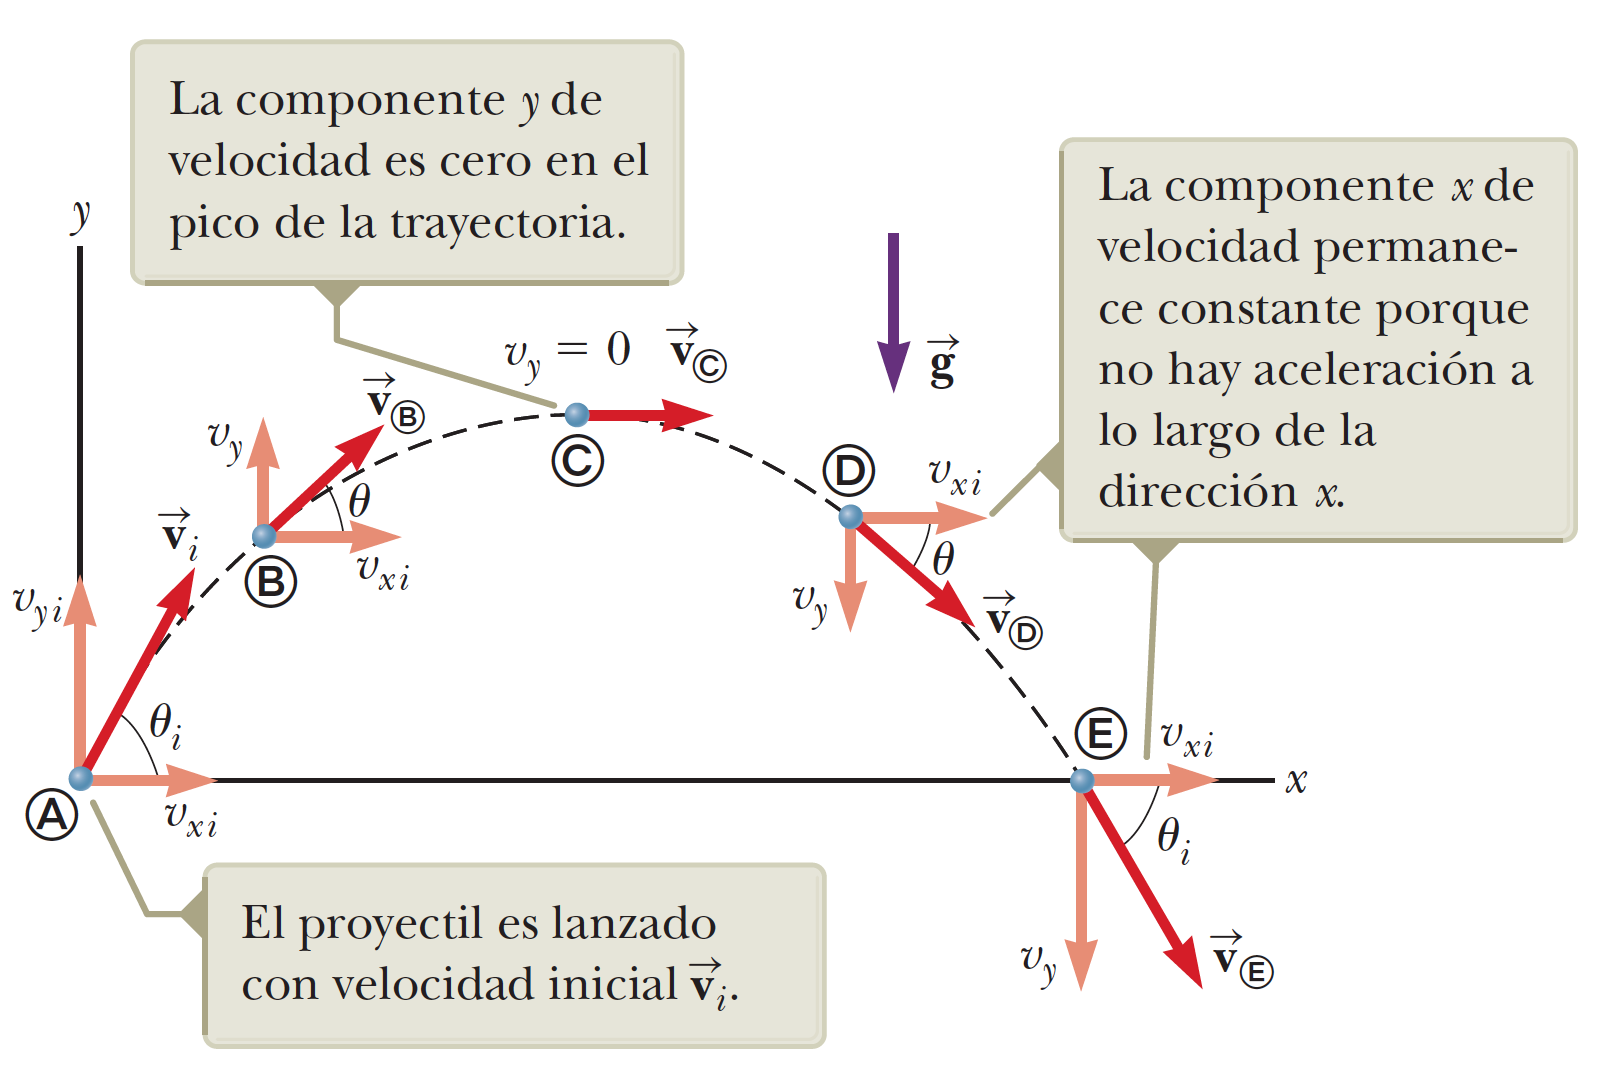
\includegraphics[scale=0.35]{1/graphics_4/figure_2}
      \caption{Trayectoria parabólica de un proyectil que sale del origen con velocidad $\BV{v}_{i}$. El vector
      velocidad $\BV{v}$ cambia con el tiempo tanto en magnitud como en dirección. Este cambio es el resultado de la
      aceleración $\BV{a} = \BV{g}$ en la dirección y negativa.}
    \end{figure}

  \subsection{Análisis de modelo: partícula en movimiento circular uniforme}
    \PN Una partícula que se mueve en una trayectoria circular con \textit{rapidez constante} v, recibe el nombre de
    \textbf{movimiento circular uniforme}. El \textbf{vector velocidad} siempre es tangente a la trayectoria del objeto
    y perpendicular al radio de la trayectoria circular, por lo tanto, siempre está cambiando la dirección del vector
    velocidad. El \textbf{vector aceleración} en movimiento circular uniforme siempre es perpendicular a la trayectoria
    y siempre apunta hacia el centro del círculo.

    \begin{figure}[H]
      \centering
      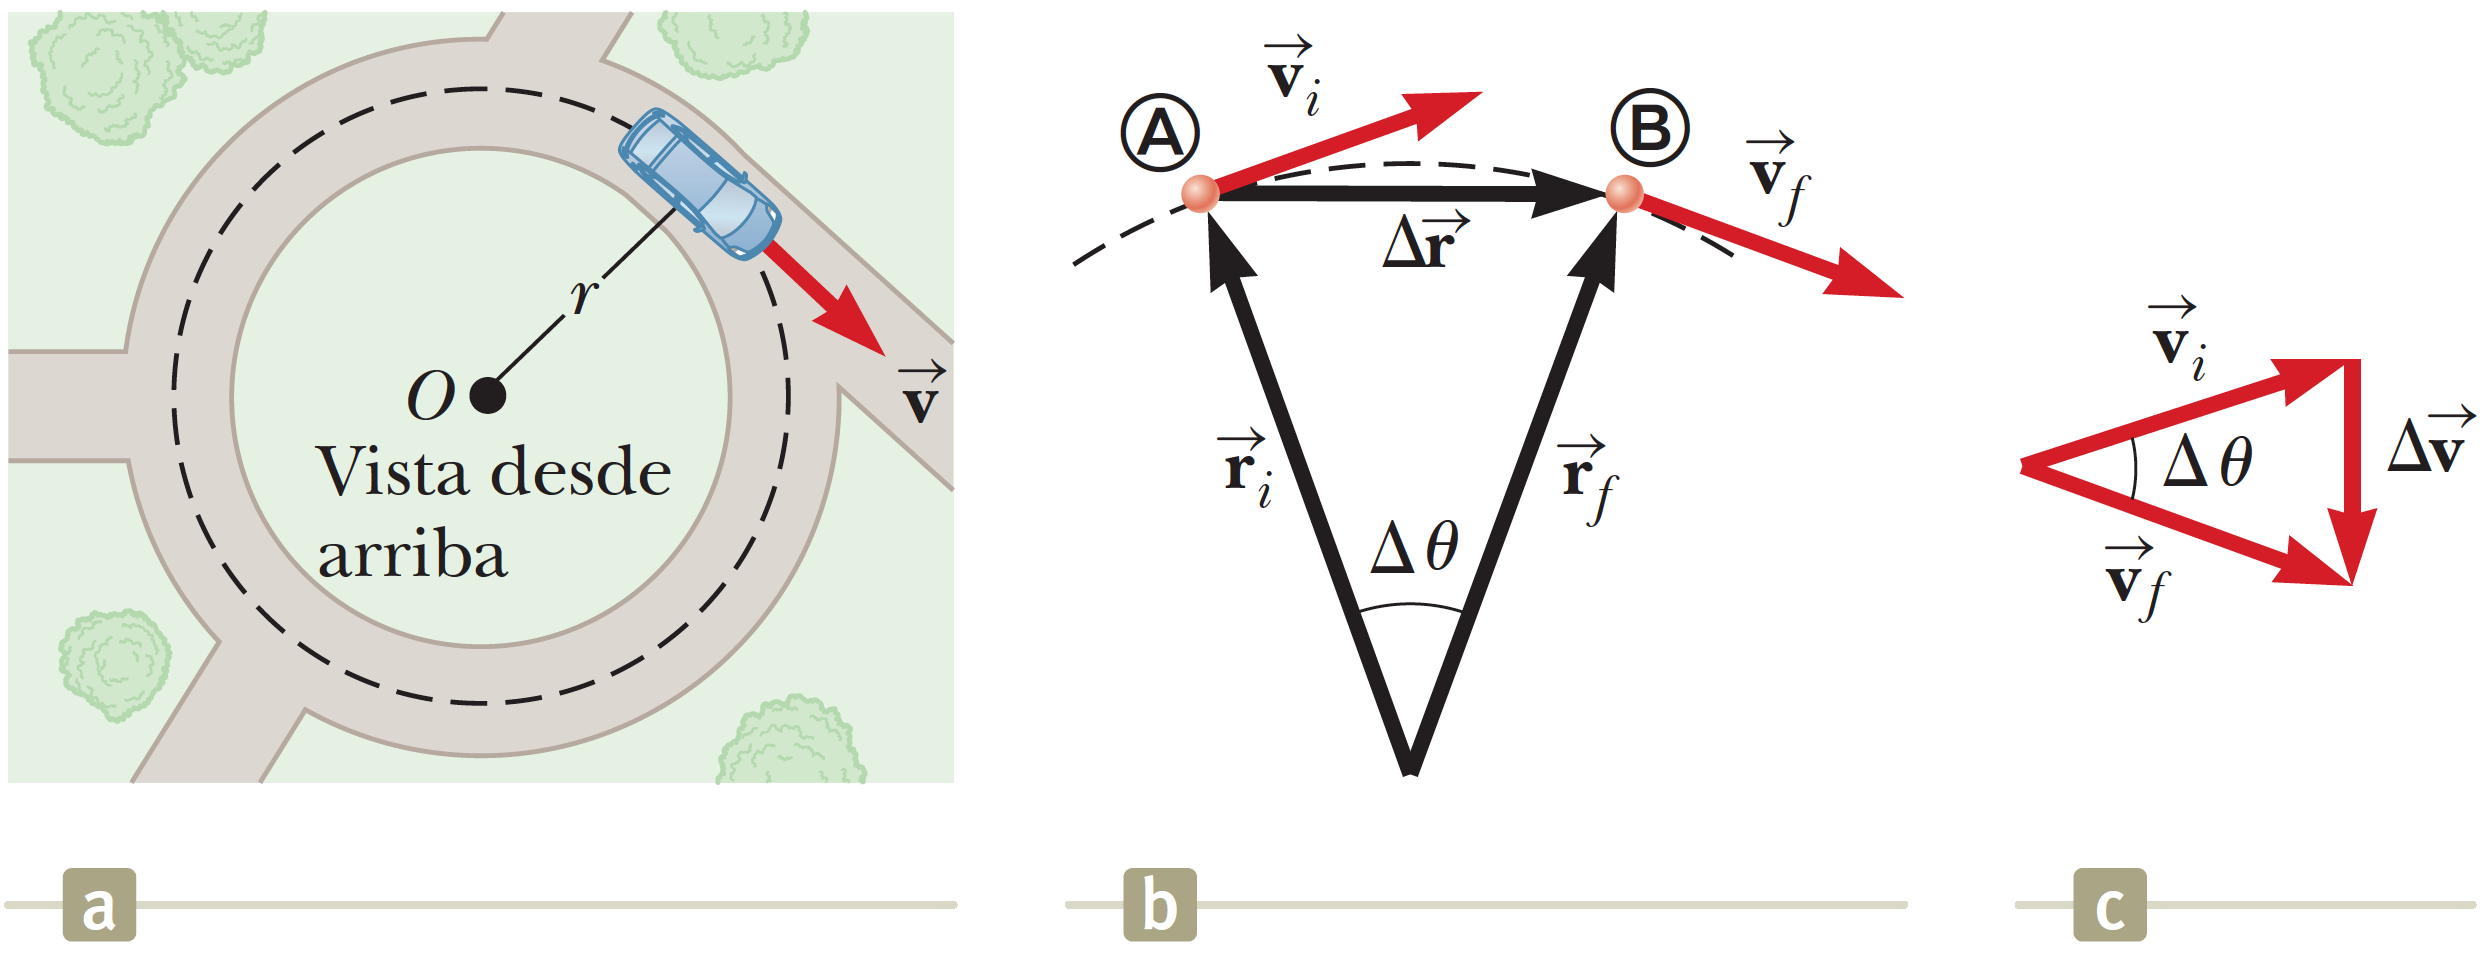
\includegraphics[scale=0.25]{1/graphics_4/figure_3}
      \caption{(a) Un automóvil que se mueve en una trayectoria circular con rapidez constante experimenta movimiento
      circular uniforme. (b) Conforme una partícula se mueve de (A) a (B), su vector velocidad cambia de $\BV{v}_{i}$ a
      $\BV{v}_{f}$. (c) Construcción para determinar la dirección del cambio en velocidad $\Delta \BV{v}$, que es hacia
      el centro del círculo para $\Delta \BV{r}$ pequeño.}
    \end{figure}

  \subsection{Acelereaciones tangencial y radial}
